\documentclass[10pt,a4paper]{article}
\newcommand{\judul}{Gerak lurus}
\newcommand{\penulis}{arifstwan}
\usepackage[latin1]{inputenc}
\usepackage{ragged2e}
\usepackage{soul}
\usepackage{amsmath}
\usepackage{microtype}
\usepackage[none]{hyphenat}
\usepackage{verbatim}
\usepackage{amsfonts}
\usepackage{amssymb}
\usepackage{enumitem}
\renewcommand{\familydefault}{\sfdefault}
\usepackage{mathpazo}
\renewcommand{\rmdefault}{put}
\usepackage{enumitem}
\usepackage[dvipsnames,svgnames]{xcolor}
\usepackage{tkz-euclide}
\usetkzobj{all}
\usepackage{graphicx}
\usepackage{fancyhdr}
\usepackage{tikz} 	
\usepackage{adjustbox}
\usepackage{multicol}
\usepackage{lipsum}
\usepackage[paperwidth=16.4cm,paperheight=21.6cm,headsep=0.2cm,footskip=0.5cm,left=0.3cm,right=0.7cm,top=1.7cm,bottom=1.0cm]{geometry}
\usepackage{cancel} \usepackage{xcolor}
\usepackage{tcolorbox}
\usetikzlibrary{decorations.pathmorphing,patterns}
\usetikzlibrary{decorations.pathreplacing,calc}
 \newcommand\coret[2][red]{\renewcommand\CancelColor{\color{#1}}\cancel{#2}}
\SetLabelAlign{Center}{\hfil\makebox[1.0em]{#1}\hfil}

\newtcolorbox{mybox}[1][] { colframe = cyan!40, colback = cyan!10,boxsep=0pt,left=0.2em, coltitle = blue!20!black, title = \textbf{jawab}, #1, } 

\newtcolorbox{rumus}[1][] { colframe = blue!10, colback = blue!3,boxsep=0pt,left=0.2em, coltitle = blue!20!black, title = \textbf{Rumus}, #1, } 
%---------- kunci (jika 1 ) muncul
\def\tampilkunci{1}
\newcommand{\hide}[1]{\ifnum\tampilkunci=1
%
\begin{mybox}
 #1
\end{mybox}
%
%\vspace{\baselineskip}
\fi}
\newcommand{\unhide}[1]{
\begin{mybox}
#1\end{mybox}}


\newtcbox{\rumuskecil}[1][red]{on line,
arc=7pt,colback=#1!10!white,colframe=#1!50!black,
before upper={\rule[-3pt]{0pt}{10pt}},boxrule=1pt,
boxsep=0pt,left=6pt,right=6pt,top=2pt,bottom=2pt}
\newtcolorbox{catatan}[1][]{%
  colback=blue!10!white, sharp corners, % No rounded corners
  boxrule=0pt, % no real frame,
  fonttitle={\large\bfseries},
  coltitle={black},  % Black colour for title
  title={ },  % Fixed title
  attach title to upper, % Move the title into the box
  #1
}


\newcommand*\cicled[1]{\tikz[baseline=(char.base)]{\node[white, shape=circle, fill=red!80,draw,inner sep=0.5pt](char){#1};}}

\newcommand*\kunci[1]{\ifnum\tampilkunci=1
%
\tikz[baseline=(char.base)]{\node[red, shape=circle,draw,inner sep=0.5pt,xshift=2pt](char){#1};}\stepcounter{enumii}
\fi\ifnum\tampilkunci=0
%
\hspace{3pt}#1\stepcounter{enumii}
%
\fi}

%------------- MULAI FUNGSIKU ------------
\newcommand{\cartesius}[3]{
\draw[help lines] (-1,-1) grid (#1);
\foreach \x in {1,2,...,#2}{
\node at (\x,0)[scale=0.5]{\x};}
\foreach \y in {1,2,...,#3}{
\node at (0,\y) [scale=0.5]{\y};}}

\newcommand{\pers}[1]{\begin{align*} #1 \end{align*}}
% \sci{ }  misal  x 10^2  tinggal tulis 
% \sci{2} 
\newcommand{\sci}[1]{$\times 10^{#1}$}

\newcommand{\scip}[1]{\times 10^{#1}}

%----membuat tanda silang di samping text
\newcommand*\silang[1]{\tikz[baseline=(char.base)]{
\draw[red,thick](-0.2,-0.20)--(0.2,0.2);
\draw[red,thick](-0.2,0.20)--(0.2,-0.2);
\node[black](char){#1};
}}
%----- membuat tanda centang di mana saja
\newcommand*\centang[1]{\tikz[baseline=(char.base)]{
\draw[red, very thick](-0.2,0.1)--(-0.1,0)--(0.2,0.3);
\node(char){#1};
}}
%------------mewarnai text merah
\newcommand*\merah[1]{
\textcolor{red}{#1}}
\newcommand*\pilgan[1]{
\begin{enumerate}[label=\Alph*., itemsep=0pt,topsep=0pt,leftmargin=*,align=Center] #1 
\end{enumerate}}

%---- membuat pernyataan pada soal SBMPTN
\newcommand*\pernyataan[1]{
\begin{enumerate}[label=(\arabic*), itemsep=0pt,topsep=0pt,leftmargin=*] #1 
\end{enumerate}}

%------ lebar baris pada tabular
\newcommand{\baris}[1]{\renewcommand\arraystretch{#1} }
%\newcommand{\tabel}[2j]{\begin{tabular}{#1}
%\end{tabular}
%------------ END OF FUNGSIKU ----------- 

\newcommand{\pilgani}[1]{
\vspace{-0.3cm}\begin{multicols}{2}
 \begin{enumerate}[label=\Alph*., itemsep=0pt,topsep=0pt,leftmargin=*,align=Center]#1
\end{enumerate}
\phantom{ini cuma sapi, wedus, dan ayam}
\end{multicols}}

%--------------- begin{document}-----------
\pagestyle{fancy}
\fancyhf{} 
\rhead{\penulis}
\lhead{\judul}
\rfoot{Hal \thepage}
\begin{document}
\begin{multicols*}{2}\centering{\textbf{FLUIDA DINAMIS}}
\begin{catatan}\textbf{A. Kontinuitas}\end{catatan}
\begin{itemize}[itemsep=0mm,topsep=0mm,leftmargin=*]
\item \textbf{Debit} (Q) adalah banyaknya Volume yang dialirkan dalam tiap satuan waktu. 

\begin{rumus}
$$ Q_1 = Q_1 $$
$$A_1.v_1 = A_2.v_2$$
\begin{tabular}{lll}
$v_1$ &:&kecepatan penampang 1 (m/s) \\
$v_t$ &:&kecepatan penampang 2 (m/s) \\
$A_1$ &:&Luas permukaan penampang 1 (m$^2$) \\
$A_2$ &:&Luas permukaan penampang 2 (m$^2$) \\
\end{tabular}
\end{rumus}

\end{itemize}

\begin{catatan}
\textbf{B. Hukum Bernoulli}
\end{catatan}
\begin{itemize}[itemsep=0mm,topsep=0mm,leftmargin=*]
\item \textbf{Percepatan} $a$ adalah perubahan kecepatan per satuan waktu $$a = \frac{\vec{v}}{t}$$

\item \textbf{Grafik} tentang GLBB misalnya tentang hubungan ($v-t$) 
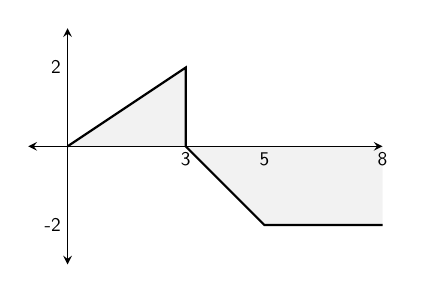
\begin{tikzpicture}[scale=0.5]
\fill [gray!10](0,0) -- (3,2)--(3,0)--cycle;
\fill [gray!10] (3,0)--(5,-2)--(8,-2)--(8,0)--cycle;
\draw[stealth-stealth] (0,3)--(0,-3);
\draw[stealth-stealth](-1,0)--(8,0);
\draw [thick](0,0)--(3,2)--(3,0)--(5,-2)--(8,-2);
\node at (3,0) [below,scale=0.7]{3};
\node at (5,0) [below,scale=0.7]{5};
\node at (8,0) [below,scale=0.7]{8};
\node at (0,2) [left,scale=0.7]{2};
\node at (0,-2) [left,scale=0.7]{-2};
\end{tikzpicture}
\begin{itemize}[label=*, topsep=0mm, itemsep=0mm]
\item Untuk menghitung jarak = luas semua arsiran (abu)
\item Perpindahan = luas di atas - luas di bawah 
\end{itemize}

\item Tiga rumus pada GLBB yang harus dihafalkan 
\renewcommand{\arraystretch}{1}
\begin{rumus}\begin{tabular}{ll}
(1) &$\vec{v_t}=\vec{v_o} +a.t$ \\
(2) &\phantom{$_t$}$\vec{s} = \vec{v_o}.t + \frac{1}{2}a.t^2$\\
(3) &${v_t}^2-{v_o}^2= 2.a.\vec{s}$\\
\end{tabular}
 

\begin{tabular}{lll}
$v_o$ &:&kecepatan awal (m/s) \\
$v_t$ &:&kecepatan akhir (m/s) \\
$a$ &:& percepatan (+) jika searah gerak\\
$\vec{s}$ &:& perpindahan (+) jika searah gerak (m) \\
\end{tabular}
\end{rumus}
\item Rumus di atas, digununakan sesuai denga kebutuhan. Misal jika tidak diketahui waktu, dan tidak perlu dicari, maka gunakan rumur (3). Sedangkan pada soal yang tidak ada hubungannya dengan perpindahan/jarak maka gunakan rumus (1), dan seterusnya
\item Pada GLBB, perlambatan artinya adalah $a$ yang bernilai negarif

\item Benda yang menjadi berhenti artinya $v_t$ adalah 0 m/s

\end{itemize}

\begin{catatan}\textbf{C. Gerak Vertikal}\end{catatan}
\textbf{Gerak Vertikal dibagi menjadi:}
\begin{enumerate}[label=\Alph*.,topsep=0mm,leftmargin=*]
\item \textbf{\textcolor{cyan}{Jatuh bebas}}

Ciri dari gerak jatuh bebas adalah "mula-mula diam","dilepas tanpa kecepatan awal", "dilepas dari ketinggian", yang semuanya mempunyai makna \textbf{$v_o=0$}. Perhatikan ilustrasi berikut:

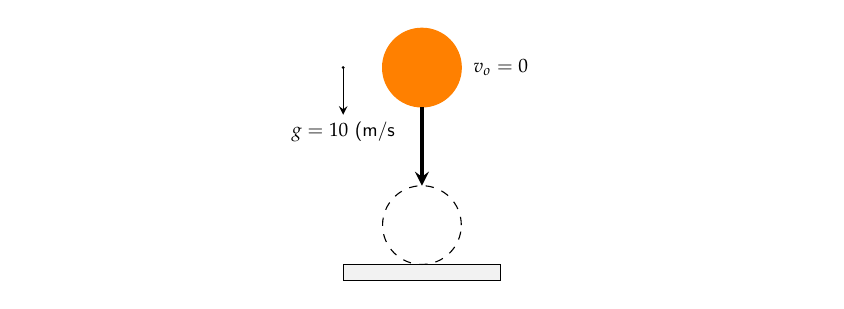
\begin{tikzpicture}
\draw [white](-5,0)--(5,0);
\draw[orange, fill=orange] (0,0) circle (0.5cm);
\draw[very thick,-stealth] (0,-0.5) --(0,-1.5);
\draw[fill=gray!10] (-1,-2.5) rectangle (1,-2.7);
\draw [dashed] (0,-2) circle (0.5);
\node at (1,0) [scale=0.7]{$v_o=0$};
\draw [fill=black](-1,0) circle(0.1mm);
\draw [-stealth] (-1,0) -- (-1,-0.6) node [below,scale=0.7]{$g=10$ (m/s};
\end{tikzpicture}

Pada kondisi ini, kecepatan awal $v_o$ = 0m/s, dan percepatan $a$ diganti dengan $+g$ yakni 10 m/s$^2$. Dan berlaku rumus 
\begin{center}
\rumuskecil[cyan]{$v=\sqrt{2gh}$} \rumuskecil[gray]{$t=\sqrt{\frac{2h}{g}}$} 
\end{center}
\item \textbf{\textcolor{cyan}{Vertikal Ke bawah}}
Pada gerak vertikal ke bawah, persamaan (1),(2), dan (3) GLBB digunakan secara utuh. esarnya $a=+g$ dan kecepatan awal $v_o$ diketahui pada soal.

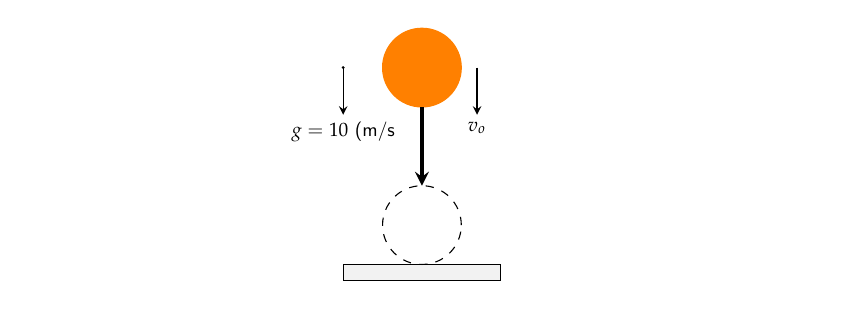
\begin{tikzpicture}
\draw [white](-5,0)--(5,0);
\draw[orange, fill=orange] (0,0) circle (0.5cm);
\draw[very thick,-stealth] (0,-0.5) --(0,-1.5);
\draw[fill=gray!10] (-1,-2.5) rectangle (1,-2.7);
\draw [dashed] (0,-2) circle (0.5);
\draw [-stealth](0.7,0)--(0.7,-0.6) node [below, scale=0.7]{$v_o$};
\draw [fill=black](-1,0) circle(0.1mm);
\draw [-stealth] (-1,0) -- (-1,-0.6) node [below,scale=0.7]{$g=10$ (m/s};
\end{tikzpicture}
\begin{center}
\rumuskecil[cyan] {$\vec{v_t}=\vec{v_o} +g.t$}\rumuskecil[gray]{$\vec{s} =\vec{h}= \vec{v_o}.t + \frac{1}{2}g.t^2$}\rumuskecil[cyan]{${v_t}^2-{v_o}^2= 2.g.\vec{h}$}
\end{center}



\item \textcolor{cyan}{\textbf{Dilempar ke atas hingga berhenti}}
Pada kasus ini benda mempunyai kecepatan mula-mula. Namun kecepatan benda berkurang karena $a$ berlawanan dengan kecepatan awal (\textbf{$a=-g$}). Sedangkan pada titik tertinggi, kecepatan benda adalah nol ($v_t=0$). Berikut ilustrasinya

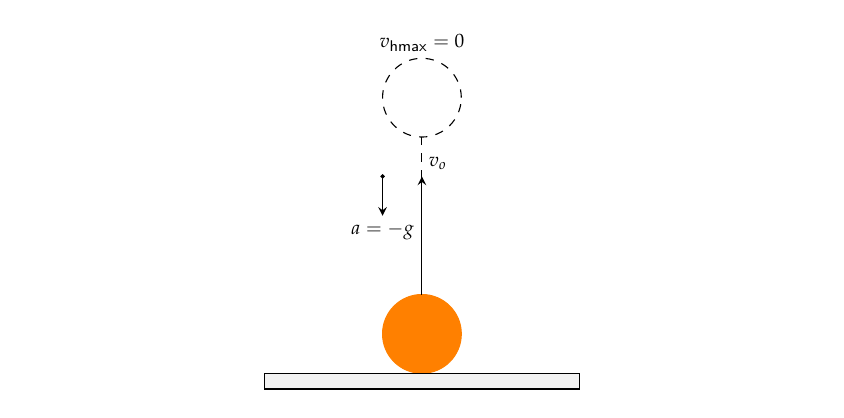
\begin{tikzpicture}
\draw [white](-5,0)--(5,0);
\draw[orange, fill=orange] (-0,0.5) circle (0.5cm);
\draw[dashed](-0.,1)--(-0.,3.);
\draw [dashed] (0,3.5) circle (0.5);
\draw [-stealth](-0,1)--(-0,2.5) node [above right, scale=0.7]{$v_o$};
\draw [fill=black](-0.5,2.5) circle(0.2mm);
\draw [-stealth] (-0.5,2.5) -- (-0.5,2) node [below,scale=0.7]{$a=-g$};
\node at (0,4)[above,scale=0.7]{$v_{\text{hmax}}=0$ };
\draw[fill=gray!10](-2,0)rectangle (2,-0.2);
\end{tikzpicture}

Karena di ketinggian maksimal kecepatan nol, maka berlaku pula persamaan

\begin{center}
\rumuskecil[cyan]{$v=\sqrt{2gh}$} \rumuskecil[gray]{$t=\sqrt{\frac{2h}{g}}$} 
\end{center}



\item \textcolor{cyan}{\textbf{Verktikal ke atas}}
Keadaan ini merupakan kebalikan dari kondisi gerak vertikal ke bawah. Gerak vertikal ke atas, menggunakan persamaan glbb (1), (2), dan (3) secara utuh, namun rumusnya diubah pada bagian $a$ menjadi $-g$


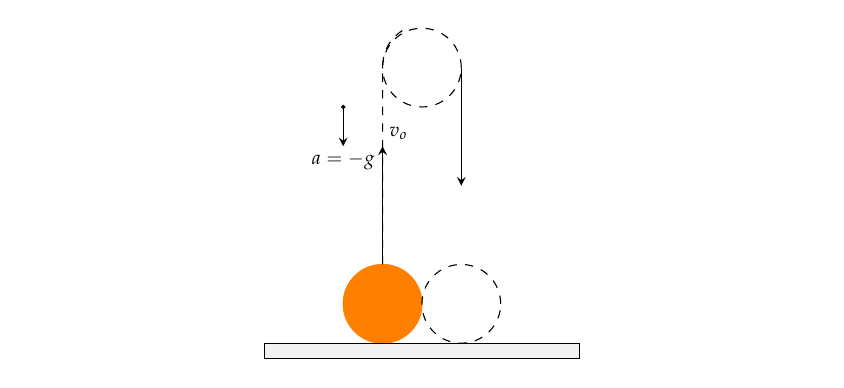
\begin{tikzpicture}
\draw [white](-5,0)--(5,0);
\draw[orange, fill=orange] (-0.5,0.5) circle (0.5cm);
\draw[dashed](-0.5,1)--(-0.5,3.5)to[bend left] (-0.2,4);
\draw[-stealth] (0.5,3.5) --(0.5,2);
\draw[fill=gray!10] (-2,0) rectangle (2,-0.2);
\draw [dashed] (0.5,0.5) circle (0.5);
\draw [-stealth](-0.5,1)--(-0.5,2.5) node [above right, scale=0.7]{$v_o$};
\draw [fill=black](-1,3) circle(0.2mm);
\draw [-stealth] (-1.,3) -- (-1.,2.5) node [below,scale=0.7]{$a=-g$};
\draw[dashed](0,3.5) circle (0.5cm);

\end{tikzpicture}

\begin{center}
\rumuskecil[cyan] {$\vec{v_t}=\vec{v_o} -g.t$}\rumuskecil[gray]{$\vec{s} =\vec{h}= \vec{v_o}.t - \frac{1}{2}g.t^2$}\rumuskecil[cyan]{${v_t}^2-{v_o}^2= 2.(-g).\vec{h}$}
\end{center}

\end{enumerate}

\begin{catatan}\textbf{Contoh Soal dan Penyelesaian}\end{catatan}
\textbf{A. GLB}
\begin{enumerate}[topsep=0pt,itemsep=0pt,leftmargin=*]
\item Dua buah mobil bergerak ke arah yang sama. Jik mobil A bergerak dengan kecepatan 20 m/s dan mobil B bergerak 50 m/s. Mobil A 150 detik lebih awal bergerak. Kapan mobil B akan menyusul mobil A?

\unhide{
\begin{tabular}{ll}
$v_A$ = 20 m/s & $v_B$ = 50 m/s \\
$t_A$ = 150s &  \\
Ditanya & $t$ saat menyusul A? \\
\end{tabular}
Pada saat A bergerak selama 150 detik, jarak yang ditempuh adalah
$$s= v.t = 20.150 = 3000\text{ m}$$
Kemudian berdasarkan catatan sebelumnya, waktu yang diperlukan untuk menyusul adalah
\begin{align*}
t&=\frac{s}{\Delta v} \\
t&=\frac{3000}{50-20}\\
t&=100 \text{ s}
\end{align*}
Berarti waktu yang diperlukan B untuk mengejar adalah 100s, atau 100+150=350s sejak A bergerak.}

\item Budi bergerak dari posisi A (0,0) ke titik B (4,0) selama 2 detik. Kemudian ke posisi (4,3) selama 6 detik. Tentukan
\begin{enumerate}[itemsep=0pt, topsep=0pt,label=\alph*.]
\item Kecepatan dari titik A ke B
\item Kelajuan dari titik A ke B
\item kecepatan dari titik A ke C
\item kelajuan dari titik A ke C
\end{enumerate}
\unhide{
\begin{enumerate}[itemsep=0pt, topsep=0pt,label=\alph*.]
\item kecepatan dari titik A ke B adalah $\vec{v}=\frac{\vec{s}}{t}=\frac{4}{2}=2 \text{ satuan/s}$
\item kelajuan dari titik A ke B adalah $v=\frac{s}{t} = \frac{4}{2} =2$ satuan/s
\item kecepatan dari titik A ke C adalah $\vec{v}=\frac{\vec{s}}{t}=\frac{5}{8}$ satuan/s
\item kelajuan dari titik A ke C adalah $v=\frac{s}{t}=frac{7}{8}$ satuan/s;
\end{enumerate}
}
\item Duah buah mobil terpisah pada jarak 560 meter bergerak saling mendekati pada saat yang bersamaan masing-masing bergerak lurus beraturan. Mobil pertama mula-mula berada di A bergerak lurus beraturan dengan kecepatan 144 km/jam dan mobil kedua mula-mula di B bergerak dengan kecepatan 108 km/jam.
  \begin{enumerate}[label=\alph*,topsep=0pt,itemsep=0pt]
  \item Kapan kedua mobil itu berpapasan.

  \item Pada jarak berapa dari A kedua mobil itu berpapasan?
   \end{enumerate}
\unhide{
Dari soal diketahui bahwa $v_A=144$ km/jam=$\frac{144}{3,6}= 40$ m/s

Sedangkan kecepatan $v_B=108$ km/jam=$\frac{108}{3,6}=30$ m/s
	\begin{enumerate}[label=\alph*,topsep=0pt,itemsep=0pt]
	\item waktu berpapasan $t$ 
	\begin{align*}
	t&=\frac{s}{v_1+v_2}\\
	t&=\frac{560}{30+40}=\frac{560}{70}=8\text{ s}
	\end{align*}
	\item Jarak dari A saat berpapasan adalah 
	\begin {align*}
	s_A &= v_A.t\\
	s_A &= 40.8 = 320 \text{ m}	
	\end{align*}
	\end{enumerate}
	}
\item  Sebuah benda bergerak lurus ke arah timur dengan kecepatan 5 m/s selama 10 sekon, kemudian berbalik ke arah barat lurus dengan kecepatan 10 m/s selama 2 sekon. Besarnya jarak dan perpindahan benda berturut-turut adalah. . . .  
\pilgani{
\item 30 m dan 70 m
\item 70 m dan 30 m
\item 60 m dan 90 m
\item 90 m dan 60 m
\item 100 m dan 30 m
}
\unhide{
Jarak adalah seluruh lintasan yang ditempuh

$s$ = $s_{\text{ke timur}} + s_{\text{ke barat}} = v_1.t_1 +v_2.t_2=5.10+10.2=70$ m

Perpindahan adalah selisih posisi akhir-posisi awal. Misal awal berada di titik 0,0 maka benda tersebut di akhir berada di

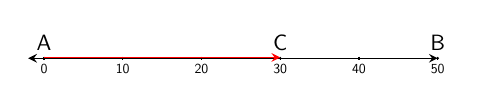
\begin{tikzpicture}[scale=0.1]
\draw[stealth-stealth](-2,0)--(50,0);
\foreach \x in {0,10,20,...,50}{
\draw(\x,0.2)--(\x,-0.2);
\node at (\x,-0.2) [below, scale=0.5]{\x};}
\draw (0,0) circle (0.7mm);
\node at (0,0) [above,scale=0.8]{A};
\draw (50,0) circle (0.7mm);
\node at (50,0) [above,scale=0.8]{B};
\draw (30,0) circle (0.7mm);
\node at (30,0) [above,scale=0.8]{C};
\draw [red,-stealth](0,0.1)--(30,0.1);
\end{tikzpicture}

Jadi perpindahan adalah posisi C - A = (3,0)--(0,0) = 30 m
}

\item Pencuri (A) mengejar polisi yang berjarak 240m. Jika polisi (B) menggunakan mobil dengan kecepatan 90 km/jam, berapakah kecepatan pencuri (A) agar dapat mengejar pada jarak 600m?
\unhide{
agar terkejar pada jarak 600m (menurut A) berarti waktu pengejaran adalah jarak/kecepatan. Jarak 600m tapi kecepatan tidak diketahui. Maka gunakan jarak yang dilalui B selama pengejaran. Kalau menurut A 600m, berarti menurut B adalah 360m lagi sampai tertangkap
$$ t = \frac{s_{\text{sisa}}}{v_B}=\frac{360}{90/3,6}=14 \text{ s}$$
Berarti dalam waktu 14 s pencuri (A) harus menempuh 600m, jadi kecepatannya
$$v_A = \frac{600}{14}=\frac{300}{7}\text{ m/s}$$}

\textbf{B. Gerak Lurus Berubah Beraturan}
\item Sebuah mobil mula-mula diam. Jika mesin dapat mempercepat 2 m/s$^2$, maka waktu yang dibutuhkan untuk mencapai 100 m adalah . . . 
\unhide{
Karena yang diketahui adalah perpindahan $\vec{s}$ dan percepatan $a$ serta yang ditanyakan adalah waktu $t$, maka rumus yang paling sesuai adalah rumus (2)
\begin{align*}
\vec{s}&=v_o.t+\frac{1}{2}a.t^2\\
100 &= 0.t + \frac{1}{2}.2.t^2\\
100 &= t^2\\
t&=\sqrt{100} = 10 \text{ s}
\end{align*}}

\item Sebuah mobil mula-mula bergerak dengan kecepatan 10 m/s. Jika perlambatan mobil adalah 4 m/s$^2$, tentukan jarak hingga berhenti.
\unhide{
\begin{tabular}{l}
$v_t$ = 0 m/s (berhenti)\\
$v_o$ = 10 m/s\\
$a$ = -4 m/s$^2$ (perlambatan)\\
ditanya: $s$ hingga berhenti . . . .?\\
\end{tabular}
Dari besaran yang diketahui, berarti rumus yang sesuai adalah rumus (3) yang tidak ada $t$
\begin{align*}
v_t^2-v_o^2 &= 2.a.s\\
0-100 &= 2.(-4).s\\
\frac{100}{8}&=s\\
s&=12,5 \text{ m}
\end{align*}
}  


\item Mobil A bergerak dengan kecepatan 40 m/s. Jika mobil B pada saat yang bersamaan mula-mula diam, dan percepatan yang dilakukan mesin adalah 2 m/s$^2$, tentukan kapan dan di mana mobil B akan menyusul A!
\unhide{
Kosep menyusul adalah jarak yang ditempuh B bisa menyamai jarak A. Padahal gerak B adalah GLBB dan gerak A adalah GLB
\begin{align*}
s_A &= s_B \\
v_A.t &= v_o.t+\frac{1}{2}.at^2\\
40t &= 0 + \frac{1}{2}.2t^2\\
40t &=t^2\\
t&=40 \text{ s} 
\end{align*}
Jadi waktu yang diperlukan untuk menyusul adalah 40 s. Adapun posisi "penyusulan" tersebut bisa dihitung dengan GLB A atau GLBB pada B.
$$s=v_A.t=40.40 =1600 \text{ m}$$
$$s=v_o.t+\frac{1}{2}a.t^2 = 0+\frac{1}{2}2.40^2 =1600 \text{ m}$$
}

\item Sebuah partikel bergerak dengan grafik hubungan kecepatan dan waktu seperti pada gambar

\begin{tikzpicture}[scale=0.6]
\draw[stealth-stealth](0,5)node[above,scale=0.7]{$v$ (m/s)} -- (0,0) -- (5,0)node[right,scale=0.7]{$t$ (s)} ;
\node at (0,1.5) [left,scale=0.7]{6};
\node at (0,4) [left,scale=0.7]{16};
\node at (4,0) [below,scale=0.]{4};
\draw[thick](0,1.5)--(4,4);
\draw [dashed] (0,4)--(4,4)--(4,0);
\end{tikzpicture}

Tentukan jarak yang ditempuh benda 4 detik pertama!
\unhide{
Pada soal seperti ini, pastikan ingat bahwa jarak = luas daerah dibawah arsinar grafik
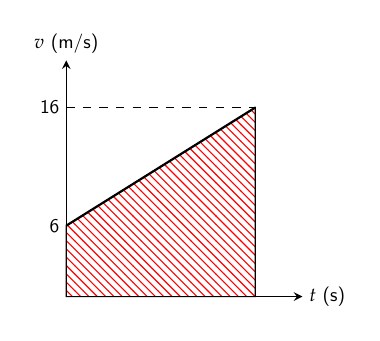
\begin{tikzpicture}[scale=0.6]
\draw[stealth-stealth](0,5)node[above,scale=0.7]{$v$ (m/s)} -- (0,0) -- (5,0)node[right,scale=0.7]{$t$ (s)} ;
\draw[pattern=north west lines, pattern color=red](0,0)--(4,0)--(4,4)--(0,1.5)--cycle;
\node at (0,1.5) [left,scale=0.7]{6};
\node at (0,4) [left,scale=0.7]{16};
\node at (4,0) [below,scale=0.]{4};
\draw[thick](0,1.5)--(4,4);
\draw [dashed] (0,4)--(4,4)--(4,0);

\end{tikzpicture}

Jadi luasnya adalah luas trapesium yakni $$L=s = \frac{(a+b)}{2}t=\frac{16+6}{2}4=44 \text{ m}$$
}

\textbf{C. Gerak Vertikal}

\item Sebuah bola dijatuhkan dari ketinggian 45 m. Tentukan berapa kecepatan di dasar sebelum menumbuk, dan berapa waktu yang diperlukan untuk mencapai tanah!
\unhide{
Karena ini adalah benda dijatuhkan berarti $v_o$ = 0 m/s berlaku
$$v = \sqrt{2gh}=\sqrt{2.10.45}=30 \text{ m/s} $$
dan
$$ t = \sqrt{\frac{2h}{g}} = \sqrt{\frac{2.45}{10}}=\sqrt{\frac{90}{10}}=\sqrt{9}=3 \text{ s}$$}


\item Sebuah benda dilemparkan ke atas dengan kecepatan awal 10 m/s. tentukan waktu agar sampai ke tanah kembali
\unhide{
cara 1

waktu hingga ke berhenti adalah
\begin{align*}
v_o&=v_o-g.t\\
t&=\frac{v_o}{g} = \frac{10}{10}=1 \text{ s}
\end{align*} 
waktu hingga ke bawah lagi adalah 2 kali waktu naik = 2 s

cara 2
perpindahan dari awal ke akhir = 0 (kembali ke tanah). Padahal $v_o$ arah ke atas dan $g$ arah ke bawah
\begin{align*}
\vec{s} &= v_o.t-\frac{1}{2}gt^2\\
0&= 10.t - 5t^2\\
10t&=5t^2 \\
t&=2\text { s}
\end{align*}}

\item Dua buah batu dilemparkan dari puncak sebuah menara pada saat yang bersamaan (g = 10 m/s$^2$). Batu pertama dilemparkan vertikal keatas dengan kecepatan 15 m/s. Sedangkan batu kedua jatuh bebas. Jarak kedua batu setelah 3 sekon adalah . . . .
\unhide{
Perlu diketahui perpindahan batu pertama $\vec{s}$. Karena berupa vektor, maka jika nilainya positif, berarti sedang berada di atas (searah dengan kecepatan), jika nilainya negatif berarti (di bawah titik awal)
\begin{align*}
\vec{s} &= v_o.t-\frac{1}{2}.g.t^2\\
\vec{s} &= 15.3 - \frac{1}{2}.10.3^2\\
\vec{2} &=45-45 =0 \text{ m}
\end{align*} 
Berarti kembali ke titik puncak menara. Mari kita hitung posisi batu kedua. Karena jatuh bebas maka $v_o=0$ dan $g=+$ (searah dengan kecepatan awal). 
\begin{align*}
\vec{s} &= v_o.t+\frac{1}{2}.10.3^2\\
\vec{s} &= 0 + 45\\
\vec{s} &= 45 \text{ m}
\end{align*}
Jadi perpindahannya sudah 45 m di bawah puncak menara. Jarak kedua batu adalah 45 m
}

\item Waktu yang diperlukan untuk jatuh bebas dari 100 m ke 20 meter adalah .. .
\unhide{
$$t=\sqrt{\frac{2h}{g}}=\sqrt{\frac{2.80}{10}}=\sqrt{16} = 4 \text{ s}$$}

\item Bola dilempar dengan kecepatan 40 m/s, waktu yang dibutuhkan untuk mencapai kecepatan maksimum adalah . .. 
\unhide{
Gunakan persamaan (1)
$$t=\frac{v_o}{g} = \frac{40}{10}=4\text{ s}$$}

\item Dari sebuah menara dengan ketinggian 70 m, batu dilempar ke atas dengan kecepatan 14 m/s. Berapa kecepatan batu saat menyentuh tanah.?

\hide{ ingat bahwa perpindahan adalah besaran vektor, maka saat dilempar ke atas, koq berakhir di bawah maka perpindahanya $\vec{s}$ = -70 m. Karena tidak mempertanyakan waktu maka hitung dengan persamaan (3)
\begin{align*}
v_t^2 - v_o^2 &= 2.a.s\\
v_t^2 - 14^2 &= 2.(-10)(-70)\\
v_t^2 &= 1400+196 = 1596 \\
v_t &= \sqrt {1596} = 39,2 \text{ m/s}
\end{align*}}


\end{enumerate}


\end{multicols*}

 \end{document}
